% ==============================================================================
% Copyright (c) 2017 [Georg R. Pollak]  
% ==============================================================================
% ------------------------------------------------------------------------------

  % Permission is hereby granted, free of charge, to any person obtaining a copy
  % of this software and associated documentation files (the "Software"), to deal
  % in the Software without restriction, including without limitation the rights
  % to use, copy, modify, merge, publish, distribute, sublicense, and/or sell
  % copies of the Software, and to permit persons to whom the Software is
  % furnished to do so, subject to the following conditions:

  % The above copyright notice, the creator of the formuary package G.R. Pollak
  % and this permission notice shall be included in all copies or substantial portions of the Software.

% ==============================================================================
% End
% ==============================================================================
% ------------------------------------------------------------------------------

% Document class
% ------------------------------------------------------------------------------
\documentclass[fourColumns]{formularyETH/formularyETH}
% formuaryETH packages
% ------------------------------------------------------------------------------
\usepackage{formularyETH/formularyETH_GeneralPackages}
\usepackage{formularyETH/formularyETH_underline}
\usepackage{formularyETH/extern/formularyETH_scientific}
\usepackage{formularyETH/extern/formularyETH_tikz}
\usepackage{formularyETH/extern/formularyETH_coding}
\usepackage{formularyETH/extern/formularyETH_algorithms}
\usepackage{formularyMacros}
% -----------------------------math Formulary----------------------------------- 
% if git@gitlab.vis.ethz.ch:formularies/math.git is used as submodule
% ------------------------------------------------------------------------------
% Uncomment next line to obtain fallback macros for math
% usepackage{math/formularyMacros} 
% Other very usefull packages
% ------------------------------------------------------------------------------
\usepackage[colorinlistoftodos,prependcaption,textsize=tiny]{todonotes}
\usepackage[skip=0pt]{caption}
\usepackage{wrapfig}
\usepackage{subcaption}
\usepackage{tabularx}
% In order to use inkscape figures with transparent fillings using alpha
\usepackage{transparent}
% -----------------------------Minted------------------------------------------- 
% minted uncomment next two lines
% ------------------------------------------------------------------------------ 
\tcbuselibrary{minted}
\tcbset{listing engine=minted}
% ------------------------------------------------------------------------------ 
% In emacs with auctex additionally add: 
% %%% TeX-command-extra-options: "-shell-escape"
% before %%% End
% -----------------------------Minted-end--------------------------------------- 
% ==============================================================================
% Documents Definitions title, date, ...
% ==============================================================================

  \title{Title}
  % Graphic-paths important when including pdf_tikz pictures e.g. with inkscape
  % ------------------------------------------------------------------------------ 
  \graphicspath{
          {figures/}
          {figures/intro/}
          %{figures/ch2/}
          }
% ==============================================================================
% Document begin
% ==============================================================================
\begin{document}
% ------------------------------------------------------------------------------ 
	\section{Introduction}
\begin{sectionbox}[\tc{optional}{Syntax}]\nospacing
  \begin{itemizenosep}
      \item \cppinline[bgcolor=mintinlinebox]/|$\alphac \optbar \betac$|/:\hfil
    either $\alphac$ or $\betac$
      \item \cppinline[bgcolor=mintinlinebox]/|$\optab{\alphac}$|/:\hfil$\alphac$ is optonal
      \item \cppinline[bgcolor=mintinlinebox]/|$\optcb{\alphac}$|/:\hfil$\alphac$ can
    occout zero or multiple times.
      \item \cppinline[bgcolor=mintinlinebox]/|$\optldots$|/:\hfil Further arguments,
    options, \ldots are possible.
  \end{itemizenosep}
\end{sectionbox}
\begin{sectionbox}[What is Java (software platform)]\nospacing
  \begin{itemizenosep}
    \item It is a high level, robust, secured and object-oriented programming
  language.
    \item Java comes with its own runtime enviroment (JRE) and API.
  Thus every hardware or software platform that supports this enviroment
  can run java programs.
  \end{itemizenosep}
\end{sectionbox}
\begin{sectionbox}[What does it consist of?]\nospacing
  \begin{itemizenosep}
      \item \imp{Java Language}: specification of the programming language.
      \item \imp{Java Virtual Machine} \imp{(JVM)}: interpreting bytecode.
      \item \imp{Java Library}: rich collection of standard APIs
    \begin{itemize}[nolistsep, noitemsep]
        \item \imp{Java Standard Edition (SE)}: is the core Java programming platform
      java.lang, java.io, java.math, java.net, java.util, etc.
        \item \imp{Java Enterprise Edition (SE)}: large scale, distributed system
      built on top of Java SE e.g. libraries for database access, remote method invocation (RMI), web services, XML,\ldots
        \item \imp{Java Micro Edition (SE)}: libraries for developing applications for mobile devices and embedded systems.
    \end{itemize}
  \end{itemizenosep}
\end{sectionbox}
\begin{sectionbox}[Features of Java]\nospacing
  \begin{itemizenosep}
      \item Object Oriented Programing (OOP) language.
      \item Platform independent.
      \item Interpreted.
      \item Multithreaded.
      \item Secured: programs run inside virtual enviroment.
      \item Automatic Garbage Collection.
  \end{itemizenosep}
\end{sectionbox}
\begin{notebox}[Why do we need yet another programming language?]\nospacing
  The problem with C/C++/\ldots is that they are designed to be compiled for
  a specific target.\\
  Eventhough its possible to compile a C++ program for just any type of CPU, to
  do so requires a full C++ compiler targeted for that CPU.\\
  \imp{Problem} writing compilers is expensive and time-consuming.\\
  \imp{Thus} the goal was to create a \imp{platform-independent language}
  that could be used to produce code that would run on a variety of CPUs under
  different enviroments.
\end{notebox}
\begin{notebox}[Types of Java Applications]\nospacing
  \begin{numberlist}
      \item \imp{Standalone Applications}: Desktop/window-based applications.
      \item \imp{Web Applications}: applications that run on the server side and
    create dynamic pages.
      \item \imp{Enterprise Applications}: are usually distributed, such as
    banking applications etc.
      \item \imp{Mobile Applications}: applications that are created for mobile
    devices e.g. Android.
  \end{numberlist}
\end{notebox}
%%% Local Variables:
%%% mode: latex
%%% TeX-master: "../formulary"
%%% TeX-command-extra-options: "-shell-escape"
%%% End:

	\section{Building a Java Program}
\begin{defnbox}\nospacing
  \begin{defn}[Compiler]
    Is a computer program (or set of programs) that translates source code of a high-level programming language, e.g. C++ into a low level language (e.g. assembly language or direct into machine language).
  \end{defn}
\end{defnbox}
\begin{defnbox}\nospacing
  \begin{defn}[Virtual Machine (VM)]
    Is a software application that simulates a computer, but hides the underlying operating system and hardware from the programs that
    interact with the VM.
  \end{defn}
\end{defnbox}
\begin{sectionbox}\nospacing
\begin{itemizenosep}
    \item \rdb{Source code} \javainline{file.java}: is first written in plain
    text files ending with a \javainline{.java} extension.\\
  \imp{Requirements}
  \begin{numberlist}
      \item Each source file can contain at most one public class.
      \item If there is a public class, then the class name and file name must match.
  \end{numberlist}
    \item \rdb{Bytecode} \javainline{file.class}: are created by the \rdb{java compiler} \tcshinline{javac.exec} from
  source code.\\
  \imp{Compiling source code}:
  \begin{mintlinebox}{java}
		javac |\opta{\optc{options}}| file.java
  \end{mintlinebox}
\end{itemizenosep}  
\end{sectionbox}
\begin{sectionbox}[\optc{Options}]\nospacing
  \begin{itemizenosep}
      \item \javainline{-d destination_folder}: compiles file into the give
    destination folder.
  \end{itemizenosep}
\end{sectionbox}
\begin{notebox}[Notes]\nospacing
  \begin{itemizenosep}
      \item Bytecode files are not files that can be read by processor of your platform yet.
      \item Bytecoes are platform-independent instructions. Thus Java's bytecode is highly portable and can run on any platform
    containg a JVM that supports the Java version of the bytecode.
  \end{itemizenosep}
\end{notebox}
\begin{defnbox}\nospacing
  \begin{defn}[Java Virtual Machine (JVM)/Interpreter]
    Is a platform independent runtime enviroment that reads and interprets the the bytecode \javainline{file.class} line by line
    in order to execute java programs.\\
    Its main tasks are: Loading the bytecode, verifying the bytecode, executing the bytecode, garbage collection,
    thread synchronization,\ldots\\
    \imp{Running Java bytecode}:\hfil \javainline{java file}
  \end{defn}
\end{defnbox}
\begin{defnbox}\nospacing
  \begin{defn}[Java Runtime Environment (JRE)]
    \imp{JVM + Libraries}:
    Provides the libraries, the Java Virtual Machine, and other components to run applets and applications
    written Java. As the JVM is just an virtual enviroment, the JRE is also known as the implementation of the JVM.\\
    It is the minimum requirement to run (not creating) java programs.
  \end{defn}
\end{defnbox}
\begin{defnbox}\nospacing
  \begin{defn}[Java Development Kit (JDK)]\leavevmode\\
    \imp{JRE + Development Tools}:
    It consits of the JRE plus tools such as compilers or debuggers for developing applets and applications.\\
    Thus is necessay in order to develope and running code.
  \end{defn}
\end{defnbox}
\begin{sectionbox}\nospacing
  \begin{figure}[H]	
    \centering{
      \vspace{-1em}
      \def\svgwidth{190pt}
      \resizebox{0.8\linewidth}{!}{\input{figures/intro/program.pdf_tex}}
    }
  \end{figure}
\end{sectionbox}
\begin{notebox}[Apllets vs. Applications]\nospacing
  All Java programs can be classified as Applications and Applets. The striking differences are that applications contain main() method where as applets do not. One more is, applications can be executed at DOS prompt and applets in a browser. We can say, an applet is an Internet application.
\end{notebox}
%%% Local Variables:
%%% mode: latex
%%% TeX-master: "../formulary"
%%% TeX-command-extra-options: "-shell-escape"
%%% End:

\section{Basics}
  \begin{sectionbox}\nospacing
  In Java, every variable, constant, and function (\textit{including main}) must
  be inside some class.\\
  \rdb{A Java Program}: is a class which contains a main method:
  \begin{mintlinebox}{java}
		public static void main(String[] args) { |\ldots| }
  \end{mintlinebox}
  \begin{itemizenosep}
      \item \javainline{pulic}: accessible from everywhere.
      \item \javainline{static}: defined on the class level (not bound to instances).
      \item \javainline{void}: does not return a result ($\Rightarrow$ procedure)
      \item \javainline{args}: argument, array of command-line arguments
  \end{itemizenosep}
\end{sectionbox}
\subsection{Packages}
\begin{sectionbox}\nospacing
  Programmers can define their own packages to bundle group of
  classes/interfaces, etc.\\
  Packages create a new namespace thus there won't be any name conflicts with
  similar identifiers from other packages.
\end{sectionbox}
\begin{defnbox}\nospacing
  \begin{defn}[Package Statement]
    Identifies the package that a Java program belongs to.
    The package statement should be the first line in the source file
    (there can be only one package statement per source file).\\
    \imp{Package Statement}:\hfil \javainline{package package-name;}
  \end{defn}
\end{defnbox}
\begin{sectionbox}[Compiling source files with package statements]\nospacing
  Using the \javainline{-d destination_fodler} option will create a folder with
  the given package name \textit{in the package statement} will be created in
  the given destination folder (if not existing), and place the complied source file
  into it.
  \begin{mintlinebox}{java}
		javac -d destination_folder file.java
  \end{mintlinebox}
\end{sectionbox}
\begin{sectionbox}[Using Packages]\nospacing
  \begin{itemizenosep}
      \item \javainline{package_name.identifier}: use fully qualified names.
    	\item \javainline{import package_name.*}: import the whole package.
    	\item \javainline{import package_name.identifier}: import certain identifiers.
  \end{itemizenosep}
\end{sectionbox}
\begin{stylebox}[The default package]\nospacing
  \begin{itemizenosep}
    \item 
  If a program does not include a package statement it belongs to the so called
  \rd{default package}, which is basically an default, unnamed package.\\
  When developing small or temporary applications e.g. for testing purposes, its
  ok not to include a package statement.\\
  \imp{But} in order to avoid name conflicts, all java source files belonging to
  a program should contain a package statement.
    \item \imp{Convention}: use your transposed internet domain name for
  uniqueness, if you have one.
    \item \imp{Lower Cases}: use lower case letters for packages in orde
      to avoid any conflicts with the names of classes and interfaces.
  \end{itemizenosep}
\end{stylebox}
%%% Local Variables:
%%% mode: latex
%%% TeX-master: "../formulary"
%%% End:

  \newpage
\section{Java}
\begin{defnbox}\nospacing
  \begin{defn}[Liskov Substitution Principle]\label{defn:}
    If S is a subtype of T, then objects of type T may be replaced with objects of type S \imp{without} altering the correctness of the program
  \end{defn}
\end{defnbox}
\begin{sectionbox}\nospacing
  \begin{wrapfigure}{r}{0.3\linewidth}
		\centering
		\vspace{-10pt}
		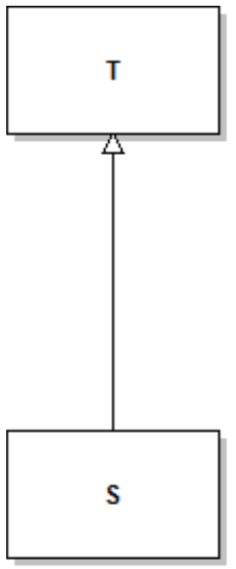
\includegraphics[width=0.55\linewidth]{figures/intro/Lis.png}
  \end{wrapfigure}
  \imp{In other words}:
  \begin{itemizenosep}
      \item Whenever you work with an instance of type T, you should not be
    surprised if you effectively work with an instance of type S
      \item An instance of type S can be used at all places where an instance of type T is expected
  \end{itemizenosep}
  \imp{Consequences}: Overriding methods need to satisfy (at least) the rules specified by the base class
\end{sectionbox}
\begin{defnbox}\nospacing
  \begin{defn}[Variance]\label{defn:Variance}
    Is a term applied to the expected behavior of subtypes in a class hierarchy containing complex types.
  \end{defn}
\end{defnbox}

%%% Local Variables:
%%% mode: latex
%%% TeX-master: "../formulary"
%%% End:

% 	\begin{sectionbox}[\subsubsection*{Variables}]\nospacing
  \begin{mintlinebox}{Java}
		Type name|\optcb{,name}|;
  \end{mintlinebox}
  \imp{Explicit Casts/Type Conversion}:
  \begin{mintlinebox}{java}
    |\optab{Type name =}| (Type) var;
  \end{mintlinebox}
\end{sectionbox}
\begin{notebox}[Note: Implicit Casts/Type Conversion]\nospacing
  \javainline/int n = 10;/\hfil\javainline/float a = n;/ $\Rightarrow$ \javainline/a = 10.0 /
\end{notebox}
%%% Local Variables:
%%% mode: latex
%%% TeX-master: "../formulary"
%%% End:
%   \subsection{Conditional Statements}
% 	\begin{sectionbox}[\subsubsection*{If}]\nospacing
  \begin{mintlinebox}{java}
		if(expression)|\optlc| statement |\optrc\opta{else \opta{if(\ldots)} statement}|
  \end{mintlinebox}
\end{sectionbox}
\begin{sectionbox}[\subsubsection*{for}]\nospacing
  \begin{mintlinebox}{java}
		for(ForControl)|\optlc| statement |\optrc|
  \end{mintlinebox}
\end{sectionbox}
\begin{sectionbox}[\subsubsection*{while}]\nospacing
  \begin{mintlinebox}{java}
		while(expression)|\optlc| statement |\optrc|
  \end{mintlinebox}
\end{sectionbox}
\begin{sectionbox}[\subsubsection*{do while}]\nospacing
  \begin{mintlinebox}{java}
		do|\optlc| statement |\optrc| while(expression);
  \end{mintlinebox}
\end{sectionbox}
\begin{sectionbox}[\subsubsection*{switch}]\nospacing
  \begin{mintlinebox}{java}
switch(expression){
  case val1: // if expression == val1
    //statemets
  break;
  case val2: // if expression == val2
    //statemets
  break;
    |\ldots|
  default:
    //statements
}
  \end{mintlinebox}
\end{sectionbox}
\begin{notebox}[Notes]\nospacing
  \begin{itemizenosep}
      \item \javainline/break;/: stops control statement at this point.
      \item \javainline/continue;/: stops control statment at this round and
    jumps to next round.
  \end{itemizenosep}
\end{notebox}
%%% Local Variables:
%%% mode: latex
%%% TeX-master: "../formulary"
%%% End:

%   \subsection{Container/Collections}
%   
%%% Local Variables:
%%% mode: latex
%%% TeX-master: "../formulary"
%%% End:

% \section{Classes}
% 	\begin{sectionbox}\nospacing
 \begin{mintlinebox}{java}
 |\opta{visibility $\optbar$ abstract}| class Name |\optla|extends BaseClass|\optra|{
   
 }|\opta{;}|
 \end{mintlinebox} 
\end{sectionbox}
\subsection{Operator Overloading}

%%% Local Variables:
%%% mode: latex
%%% TeX-master: "../formulary"
%%% End:

% \section*{Further Things}
% \subsection{JUnit}
\newpage
\section{Java}
   \appendtographicspath{
          {java/figures/}
          {java/figures/basics/}
          {java/figures/oop/}
          {java/figures/stochastic/}
          }
\section{Basics}
\begin{defnbox}\nospacing
  \begin{defn}[Resolution]
    Is a rule of inference.
  \end{defn}
\end{defnbox}
\begin{defnbox}\nospacing
  \begin{defn}[Type]\label{defn:Type}
    defines a behavior but no implementation.\\
    (Java: Types are defined by classes)
  \end{defn}
\end{defnbox}
\begin{defnbox}\nospacing
  \begin{defn}[Subtyping]\label{defn:}
    Are specializations of Types and define a \rd{is-a} relationship.\\
    (Java: Subtyping is defined by subclassing, i.e. each subclass also defines a subtype)
  \end{defn}
\end{defnbox}
\begin{defnbox}\nospacing
  \begin{defn}[Java Method Signature]\label{defn:}
    Is the method name and the number, type and order of its parameters:
    \begin{mintlinebox}{java}
      methodName(Type1, Type2,...)
    \end{mintlinebox}
  \end{defn}
\end{defnbox}
\begin{notebox}[Note]\nospacing
  Return types, name of the arguments and thrown exceptions are not considered to be a part of the method signature. 
\end{notebox}
\begin{defnbox}\nospacing
  \begin{defn}[Method Declaration]\label{defn:methodDeclaration}
  Is a declaration of a function i.e.\ declares an identifier and its types,\ldots
    \begin{mintlinebox}{java}
      visibility |\optal|static|\optar| returnType methodName (args);
    \end{mintlinebox}
  \end{defn}
\end{defnbox}
\begin{defnbox}\nospacing
  \begin{defn}[Variable\blacksl Reference Declaration]\label{defn:referenceVariable}
    In java the only way to access an object is through a reference variable.
    \begin{mintlinebox}{java}
      StaticType reference;
    \end{mintlinebox}
    A reference is not an object, thus no memory is allocated for an object of
    the Type \javainline/StaticType/.
    of the reference.
    \begin{figure}[H]
      \vspace{-5pt}
      \centering
      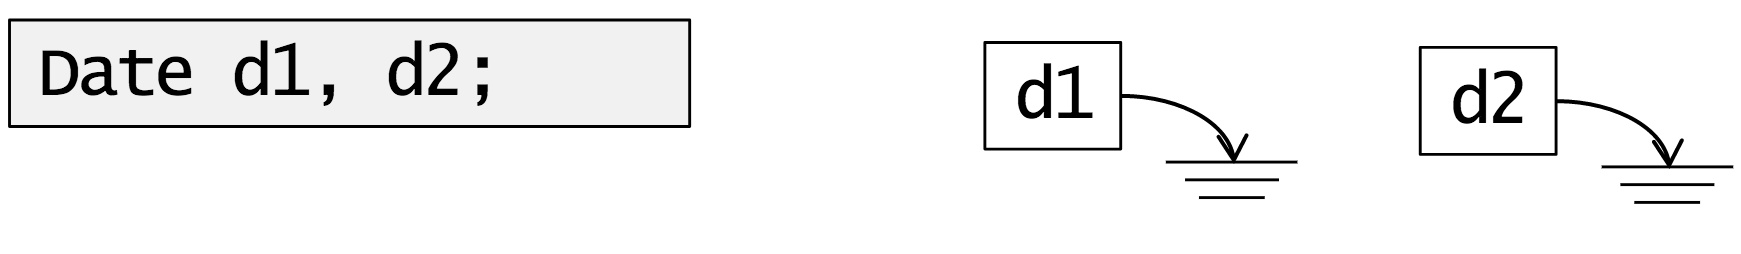
\includegraphics[width=.7\textwidth]{java/figures/basics/reference.png}
    \end{figure}
  \end{defn}
\end{defnbox}
\begin{notebox}[Note]\nospacing
  \begin{itemizenosep}
      \item Do not confuse C++ references with java references in Java variables are
  called (by convention) references.
      \item Reference variables are sort of C++ pointers but we can not do
    pointer arithmetic's on it e.g.\ \cppinline/ptr++/
      \item Reference Variables are of size:
    \begin{itemizenosep}
        \item 32-bit on a 32-bit JVM
        \item 32-bit of 64-bit on a 64-bit JVM, depending on the configuration
    \end{itemizenosep}
  \end{itemizenosep}
\end{notebox}
\begin{defnbox}\nospacing
  \begin{defn}[Static Type]\leavevmode
    A reference variable is declared to be of a specific type and that type,
    known as static type can never be changed.\leavevmode\\
    \ctr{Static type = type of reference variable}
  \end{defn}
\end{defnbox}
\begin{corbox}\nospacing
  \begin{cor}[Guarantees of Static Type]
    When a variable is declared as being of a particular type, then we have a
    language-enforced guarantee that any \textit{object} referenced by that
    reference variable will have (at least) all the features of that
    \textit{type}.\\
    $\Rightarrow$ \textit{dynamic type} needs to provide methods of \textit{static type}.
  \end{cor}  
\end{corbox}
\begin{defnbox}\nospacing
  \begin{defn}[Instanciation \javainline/new/]
    The new operator instantiates a class by dynamically allocating memory (=allocation at run time on the heap)
    for a new object and returns a reference to that memory.
    \begin{mintlinebox}{java}
      new MyClass();
    \end{mintlinebox}
    This reference can then be stored in/assigned to a (reference \cref{defn:referenceVariable}) variable.
    \begin{mintlinebox}{java}
      Type ref = new MyClass();
    \end{mintlinebox}
  \end{defn}
\end{defnbox}
\begin{notebox}[Note]\nospacing
  In Java, all class objects must be dynamically allocated.
\end{notebox}
%%% Local Variables:
%%% mode: latex
%%% TeX-master: "../../formulary"
%%% End:

\section*{Object Oriented Programming \rb{OOP}}
% ------------------------------------------------------------------------------ 
\subsection{Principles}
\begin{defnbox}\nospacing
  \begin{defn}[Encapsulation]\label{defn:encapsulation}\leavevmode
    \begin{itemizenosep}
      \item Methods and data are combined in classes
      \item Not unique to OOP
    \end{itemizenosep}
  \end{defn}
\end{defnbox}
\subsection{Class Basics}
\subsubsection{Static}
\label{subsubsec:Static}
\begin{defnbox}\nospacing
  \begin{defn}[Static Fields]\label{defn:staticFields}
    Per class fields, accessible via class (or instance)
    \begin{itemizenosep}
        \item Bound to class (available even if no instance has been created)
        \item Only one copy of the attribute (identical for all instances)
        \item Initialization per default with zero (0 / 0.0 / false / null) 
    \end{itemizenosep}
    \begin{mintlinebox}{java}
      static Type ref;
    \end{mintlinebox}
  \end{defn}
\end{defnbox}
\begin{stylebox}[Constants]\nospacing
  Declare constants as \javainline/static final/ fields.
\end{stylebox}
\begin{defnbox}\nospacing
  \begin{defn}[Static Methods]\label{defn:staticFields}
    Per Class methods, accessible via class (or instance):
    \begin{mintlinebox}{java}
      static ResultType Name(args){ Body }
    \end{mintlinebox}
    \begin{itemizenosep}
        \item No \javainline/this/
        \item No access to instance attributes \& methods
    \end{itemizenosep}
  \end{defn}
\end{defnbox}
\begin{stylebox}\nospacing
  Do not use instances to access static fields or methods.
\end{stylebox}
\subsubsection{Class Initialization}
\begin{sectionbox}[Upon loading o the class]\nospacing
  
\end{sectionbox}
\subsection{Inheritance}
\begin{defnbox}\nospacing
  \begin{defn}[\tc{black}{\normalfont{(Implementation Aspect)}}
    \\Code Inheritance\blacksl Extension\blacksl Subclassing]\leavevmode
    \begin{itemizenosep}
        \item Subclasses add new fields \& methods
        \item Subclasses have more (specialized) attributes \& operations
        \item Implementation aspect
    \end{itemizenosep}
    \imp{Class}: defines a type \imp{and} implementation
  \end{defn}
\end{defnbox}
\begin{defnbox}\nospacing
  \begin{defn}[\tc{black}{\normalfont{(Design Aspect)}}
    \\Interface Inheritance\blacksl Specialization\blacksl Subtyping]\leavevmode
    \begin{itemizenosep}
        \item Types define a set of objects
        \item Subtypes are specializations of this Type
        \item Inheritance of behavioral aspects
    \end{itemizenosep}
    \imp{Interface}: defines type
  \end{defn}
\end{defnbox}
\begin{defnbox}\nospacing
  \begin{defn}[\javainline/extends/]\label{defn:extends}\leavevmode\\
    Define new class by extending existing classes.\\
    In Java only one base class can be specified to inherit from.
    Extension inherits all fields and methods from the base class.
  \end{defn}
\end{defnbox}
\subsubsection{Polymorphism}
\begin{defnbox}\nospacing
  \begin{defn}[Type Checking]
    The process of verifying and enforcing the constraints of types
  \end{defn}
\end{defnbox}
\begin{defnbox}\nospacing
  \begin{defn}[Statically Typed Languages]
    Is a language where the type of a variable is known at compile time.\\
    For some languages this means that we as programmer must specify of what type each variable is.\\
    \Advantage\ can do type-checking during compile time by the compiler, and therefore a lot of trivial bugs are caught at a very early stage.\\
    \imp{Examples}: C, C++, Java
  \end{defn}
\end{defnbox}
\begin{defnbox}\nospacing
  \begin{defn}[Dynamically Typed Languages]
     If the type is associated with/depends on run-time \imp{values}, and not named variables/fields/etc\\
     \Advantage\ we do not have to specify types every time.\\
     \Drawback\ do type checking at run-time
  \end{defn}
\end{defnbox}
\label{subsubsec:Polymorphism}
\begin{defnbox}\nospacing
  \begin{defn}[Polymorphism]\label{defn:polymorphism}
    Polymorphism allows operations to be performed on objects without needing to know which class the object belongs to,
    provided that we can guarantee that the class implements the specified type.
  \end{defn}
\end{defnbox}
\begin{defnbox}\nospacing
  \begin{defn}[Polymorphic Assignment]
    Instances of an extended class can be assigned to references of type base
    class:
    \begin{mintlinebox}{java}
      BaseClass ref = new extendedClass();
    \end{mintlinebox}
  \end{defn}
\end{defnbox}
\begin{defnbox}\nospacing
  \begin{defn}[Dynamic Type]\label{defn:dynamicType}
    Is the type of the object assigned to a reference variable.\\
    Dynamic types of reference variables may change with every assignment.\\
    $\text{Dynamic Type}\subseteq\text{Static Type}$ as the dynamic type most
    full fill at least the guarantees of the static type.
  \end{defn}
\end{defnbox}
\begin{defnbox}\nospacing
  \begin{defn}[Static Binding]
    Is type resolution based on the static type of a variable reference.
  \end{defn}
\end{defnbox}
\begin{defnbox}\nospacing
  \begin{defn}[Static Binding and Overloading]
    If we overload a method in Java, the compiler will produce a version for
    each overloaded function \rd{signature}.\\
    The resolution of the method signature (not to the actual implementation) of the
    method is done during compile time and does hence depend on the \rd{static type}
    passed to the method $\Rightarrow$ static binding
    \begin{mintlinebox}{java}
      StaticTypeOfa a = new DynamicTypeOfa();
      a.methodToResolveTo(StaticTypeOfb b);
    \end{mintlinebox}
    \javainline/staticTypeOfb/ decides which overloaded method to call.
  \end{defn}
\end{defnbox}
\begin{defnbox}\nospacing
  \begin{defn}[\\Dynamic Type Binding and Overloading]
    The runtime chooses a function implementation
    \begin{numberlistnosep}
        \item Based on the function \rd{signature} chosen at compile time
      (dynamic binding)
        \item Depending on the dynamic type of the object referenced by
      \javainline/a/ in order to chose an actual implementation of
      \begin{mintlinebox}{java}
          DynamicTypeOfa.methodToResolveTo(StaticTypeOfb b)
      \end{mintlinebox}
    \end{numberlistnosep}
  \end{defn}
\end{defnbox}
\begin{notebox}[Note]\nospacing
  For non-overloaded methods only the dynamic type of the reference variable
  decides which method to call.
\end{notebox}
\begin{codeboxNl}[Dynamic Type Inference]{java}
  if( ref instanceof Type)
\end{codeboxNl}
\begin{codeboxcomment}[Type Casts]{0.3}{java}{
    A runtime error is thrown if the dynamic type of \javainline/ref/ is not a
    Type or extension thereof.
  }
  (Type) ref;
\end{codeboxcomment}
\subsection{Abstract Classes}
\begin{defnbox}\nospacing
  \begin{defn}[Abstract Methods]
    Are methods that only define a signature/are only a declaration:
    \begin{mintlinebox}{java}
      visibility abstract retrunType methodName();
    \end{mintlinebox}
    \begin{itemizenosep}
        \item Define methods to be implemented in subclasses
        \item Can only be declared in \javainline/abstract/ classes
        \item Cannot be \javainline/private/ as private methods cannot be overridden
        \item Cannot be \javainline/static/ as static methods cannot be overridden
    \end{itemizenosep}
  \end{defn}
\end{defnbox}
\begin{defnbox}\nospacing
  \begin{defn}[Abstract Classes]
    Are classes that how stand in an ``\rd{is-a}'' relationship with their subclasses:
    \begin{itemizenosep}
      \item Cannot be instantiated
      \item Usually have one or more abstract methods
      \item May have attributes, constructors, non-abstract methods 
    \end{itemizenosep}
    \begin{mintlinebox}{java}
      visibility abstract class Name{ Body }
    \end{mintlinebox}
  \end{defn}
\end{defnbox}
\begin{notebox}[Note]\nospacing
  An abstract class must not necessarily have an abstract method.\\
  Useful to declare classes abstract that cannot/may not be initiated but (but extended)
\end{notebox}
\begin{notebox}[Note: \normalfont{Derived Classes}]\nospacing
  \begin{itemizenosep}
      \item Have to override (implement) all \javainline/abstract/ methods
      \item Or have to be declared abstract as well, if not all abstract methods
    are overridden.
  \end{itemizenosep}
\end{notebox}
\begin{notebox}[Note]\nospacing
  Arrays of an abstract base type may be instantiated sine No instances are
  created (only reference variables)
  \begin{mintlinebox}{java}
    ContainerType[] name = new ContainerType[Number]
  \end{mintlinebox}
\end{notebox}
\begin{stylebox}[Usage]\nospacing
  \begin{itemizenosep}
      \item Want to share code among several closely related classes.
      \item You expect that classes that extend your abstract class have many
    common methods or fields or require access modifiers other than public (such
    as protected and private).
      \item You want to declare non-static or non-final fields. This enables you to define methods that can access and modify the state of the object to which they belong.
  \end{itemizenosep}
\end{stylebox}
\subsection{Interfaces}
\begin{defnbox}\nospacing
  \begin{defn}[Interfaces=pure abstract class]\label{defn:interfaces}
    Have to be implemented by the class that uses the interface and represent a
    ``\rd{can-do}'' relationship:
    \begin{itemizenosep}
      \item Have only \javainline/public/ and \javainline/abstract/ methods
      \item Attributes are by default \javainline/public,static/ and
    \javainline/final/
      \item No constructors $\Rightarrow$ instantiated ($\neq$ declared)
    \end{itemizenosep}
    \imp{Definition}:
    \begin{mintlinebox}{java}
      public intreface ClassName{ Body; }
    \end{mintlinebox}
    \imp{Implementation}:
    \begin{mintlinebox}{java}
      class ClassName implements IntefaceName{ Body; }
    \end{mintlinebox}
    \begin{itemizenosep}
        \item All methods defined in the declared interface have to be
      implemented unless its another interface adding more functionality
        \item A class may implement multiple interfaces
    \end{itemizenosep}
  \end{defn}
\end{defnbox}
\begin{notebox}[Note: Java 8 default methods]\nospacing
  Can be implemented inside interfaces and are able access other methods.
  Allows to extend interfaces without breaking existing classes that implement
  the interface.
\end{notebox}
\begin{stylebox}\nospacing
  Use \javainline/@override/ to implement the methods.
\end{stylebox}
\begin{stylebox}[Usage]\nospacing
  \begin{itemizenosep}
    \item You expect that unrelated classes would implement a piece of
  functionality. 
    \item Want to specify the behavior of a particular data type, but not concerned about who implements its behavior.
  \end{itemizenosep}
\end{stylebox}
\begin{notebox}[Interfaces as function arguments]\nospacing
  Methods with Interfaces as type can be called with any class implementation
  that interface.
\end{notebox}
\begin{notebox}[Interface Reference]\nospacing
  Interfaces can be used as reference variable for all subclasses \imp{but} be
  care-full if the reference object implements another interface we will not be
  able to call its functions unless we use an implicit cast.\\
  Check if referenced object implements an interface: \javainline/ref instanceof aInterface/
\end{notebox}
\begin{codeboxNl}[Interaface Variable]{java}
  TypeImplementingAandB ref = new TypeImplementingAandB()
  InterfaceTypeA refA = ref;
  InterfaceTypeB refB = ref;
  refA instanceof InterfaceTypeB // True as ref implements B
  refA.methodOfTypeImplementingAandB() // works
  refA.methodOfB() // does not work
  ((InterfaceTypeB)refA).methodOfB() // works
\end{codeboxNl}
\begin{sectionbox}[Intrefaces and Abstract Classes]\nospacing
  \begin{itemize}
      \item \javainline/Interface/: provides a type
      \item \javainline/abstract Class/ semi finished component that contains
    default implementations
    \begin{itemizenosep}
        \item which can be used in subclasses
        \item which can be overriden in subclasses
    \end{itemizenosep}
  \end{itemize}
  \begin{figure}[H]
    \centering
    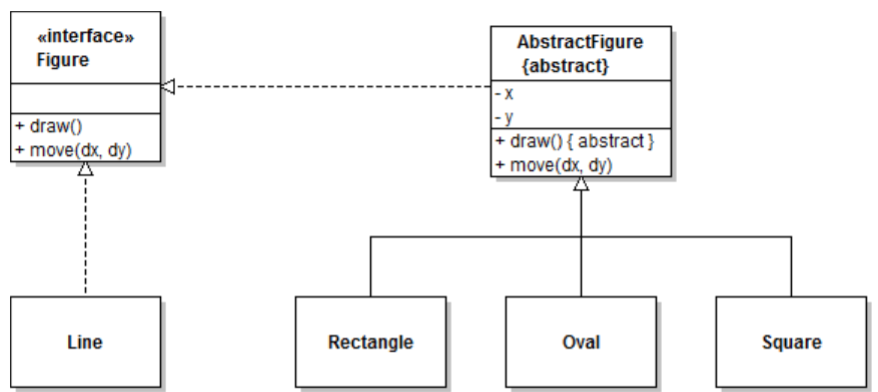
\includegraphics[width=1.0\textwidth]{java/figures/oop/abstractInterface.png}
  \end{figure}
\end{sectionbox}
\begin{notebox}[Abstract Classes vs. Interfaces]\nospacing
  \begin{itemizenosep}
      \item Abstract Classes
    \begin{itemizenosep}
        \item A class may extend only one abstract class
        \item Abstract classes may contain attributes \& concrete implementations
    \end{itemizenosep}
      \item Interfaces
    \begin{itemizenosep}
        \item A class may implement sever interfaces
        \item Abstract classes may contain no implementations 
    \end{itemizenosep}
  \end{itemizenosep}
\end{notebox}
\begin{defnbox}\nospacing
  \begin{defn}[Marker Interface]\label{defn:markerInerface}
    Is an empty interface, that can be used to add a certain
    attribute/characteristic to a class that can be checked with
    \javainline/instanceof/ e.g.\ RandomAcess 
  \end{defn}
\end{defnbox}
\begin{defnbox}\nospacing
  \begin{defn}[Functional Interface \javainline/@FunctionalInterface/]\label{defn:functionalInterface}
    Is an interface with a single abstract method:
    \begin{mintlinebox}{java}
      @FunctionalInterface
      public interface InterfaceName{
        visibility returnType methodName(args);
      }
    \end{mintlinebox}
  \end{defn}
\end{defnbox}
\begin{notebox}[Notes]\nospacing
  \begin{itemizenosep}
      \item The annotation \javainline/@FunctionalInterface/ allows compilers to generate an
  error if the interface does not satisfy the conditions of a functional
  interface.
    \item Default methods are not abstract and do not count.
  \end{itemizenosep}
\end{notebox}
\begin{sectionbox}[Lambda Expressions and Functional Interfaces]\nospacing
  
\end{sectionbox}
%%% Local Variables:
%%% mode: latex
%%% TeX-master: "../../formulary"
%%% End:

% ------------------------------------------------------------------------------ 
%%% Local Variables:
%%% mode: latex
%%% TeX-master: "../formulary"
%%% End:

\newpage
% ==============================================================================
% Design Patterns
% ==============================================================================
\section{Behavioral Patters}
\label{subsubsec:Behavirol}
\subsection{Composite}
  \subsubsection{Transparent vs.\ Safe Approach}
\begin{sectionbox}[Problem]\nospacing
  Being able to treat a heterogeneous collection of objects atomically (or transparently) requires that the "child management" interface be defined at the root of the Composite class hierarchy (the abstract Component class). However, this choice costs you safety, because clients may try to do meaningless things like add and remove objects from leaf objects. On the other hand, if you "design for safety", the child management interface is declared in the Composite class, and you lose transparency because leaves and Composites now have different interfaces.
\end{sectionbox}

%%% Local Variables:
%%% mode: latex
%%% TeX-master: "../formulary"
%%% End:

\section{Structural Patters}
\label{subsubsec:Behavirol}
\section{Creational Patters}
\label{subsubsec:Behavirol}
% ======================================================================
% Todo
% ======================================================================
\add{Method type bindining exercise 2/slides/more research}
\add{Nested Classes/Anonymous functions}
$https://www.tutorialspoint.com/java/java_innerclasses.htm$
\add{Java generics, generics with questionmark and extends.}
%%% Local Variables:
%%% mode: latex
%%% TeX-master: "../formulary"
%%% End:

  
% ==============================================================================
% Document end
% ==============================================================================
\end{document}




%%% Local Variables:
%%% mode: latex
%%% TeX-master: t
%%% TeX-command-extra-options: "-shell-escape"
%%% End:
